\documentclass[12pt, a4paper]{article}
\usepackage{latexsym, listings, graphicx, hyperref, gensymb}


\lstset{language=bash}  

\newtheorem{theorem}{Theorem}
\newtheorem{definition}{Definition}

\renewcommand{\baselinestretch}{1.3} % 1.5 denotes double spacing. Changing it will change the spacing

\setlength{\parindent}{0in} 

\begin{document}
\title{Testing hig magnification (100x) \\ on  growth
  of \\  household yeast}
\author{Bjørn Remseth}
\date{30. mar. 2016}
\maketitle
\abstract{Tried to make a movie of yeast growing under 100x magnification.  The attempt failed since the  yeast died, probably due to too high temperature of the sugar solution.}

\section{Introduction}


Used the same experimental setup as in day before yesterday's setup.   

A yeast/sugar/water solution was made by adding about a teaspoon of
sugar to an egg-glass of water and stirring.  The solution was then
cooled by adding tapwater.  To this solution a small amount (roughly
equivalent to 30 \(mm^3\) of household yeast (``IDUN mors hjemmebakte
original gjær'' with a ``best before'' marking of april 10 2016).

Used a feber termometer to determine when to add yeast.  Did it when
the temperature of the water was \(40.7 \degree C\).

A drop of this solution was put onto a microscope slide (``Elka
Assistent, Objektträger micro slides  cleaned'') and then put onto the
microscope and a cover glass was put on top.   The solution spread out
under the entire cover glass and on visual inspection it seemed to be
completely uniform.

The slide was then put onto the microscrope.  The microscope is an
Amscope 40X-2500X Infinity trinocular compound microscope.  The 100x
microscope lens (oil) was selected, and a drop of immersion oil was
added to the slide.


Identical scripts as in the previous experiments were used to create
samples and a movie of the animation.

\section{Results}

\begin{figure}[th]
\begin{center}
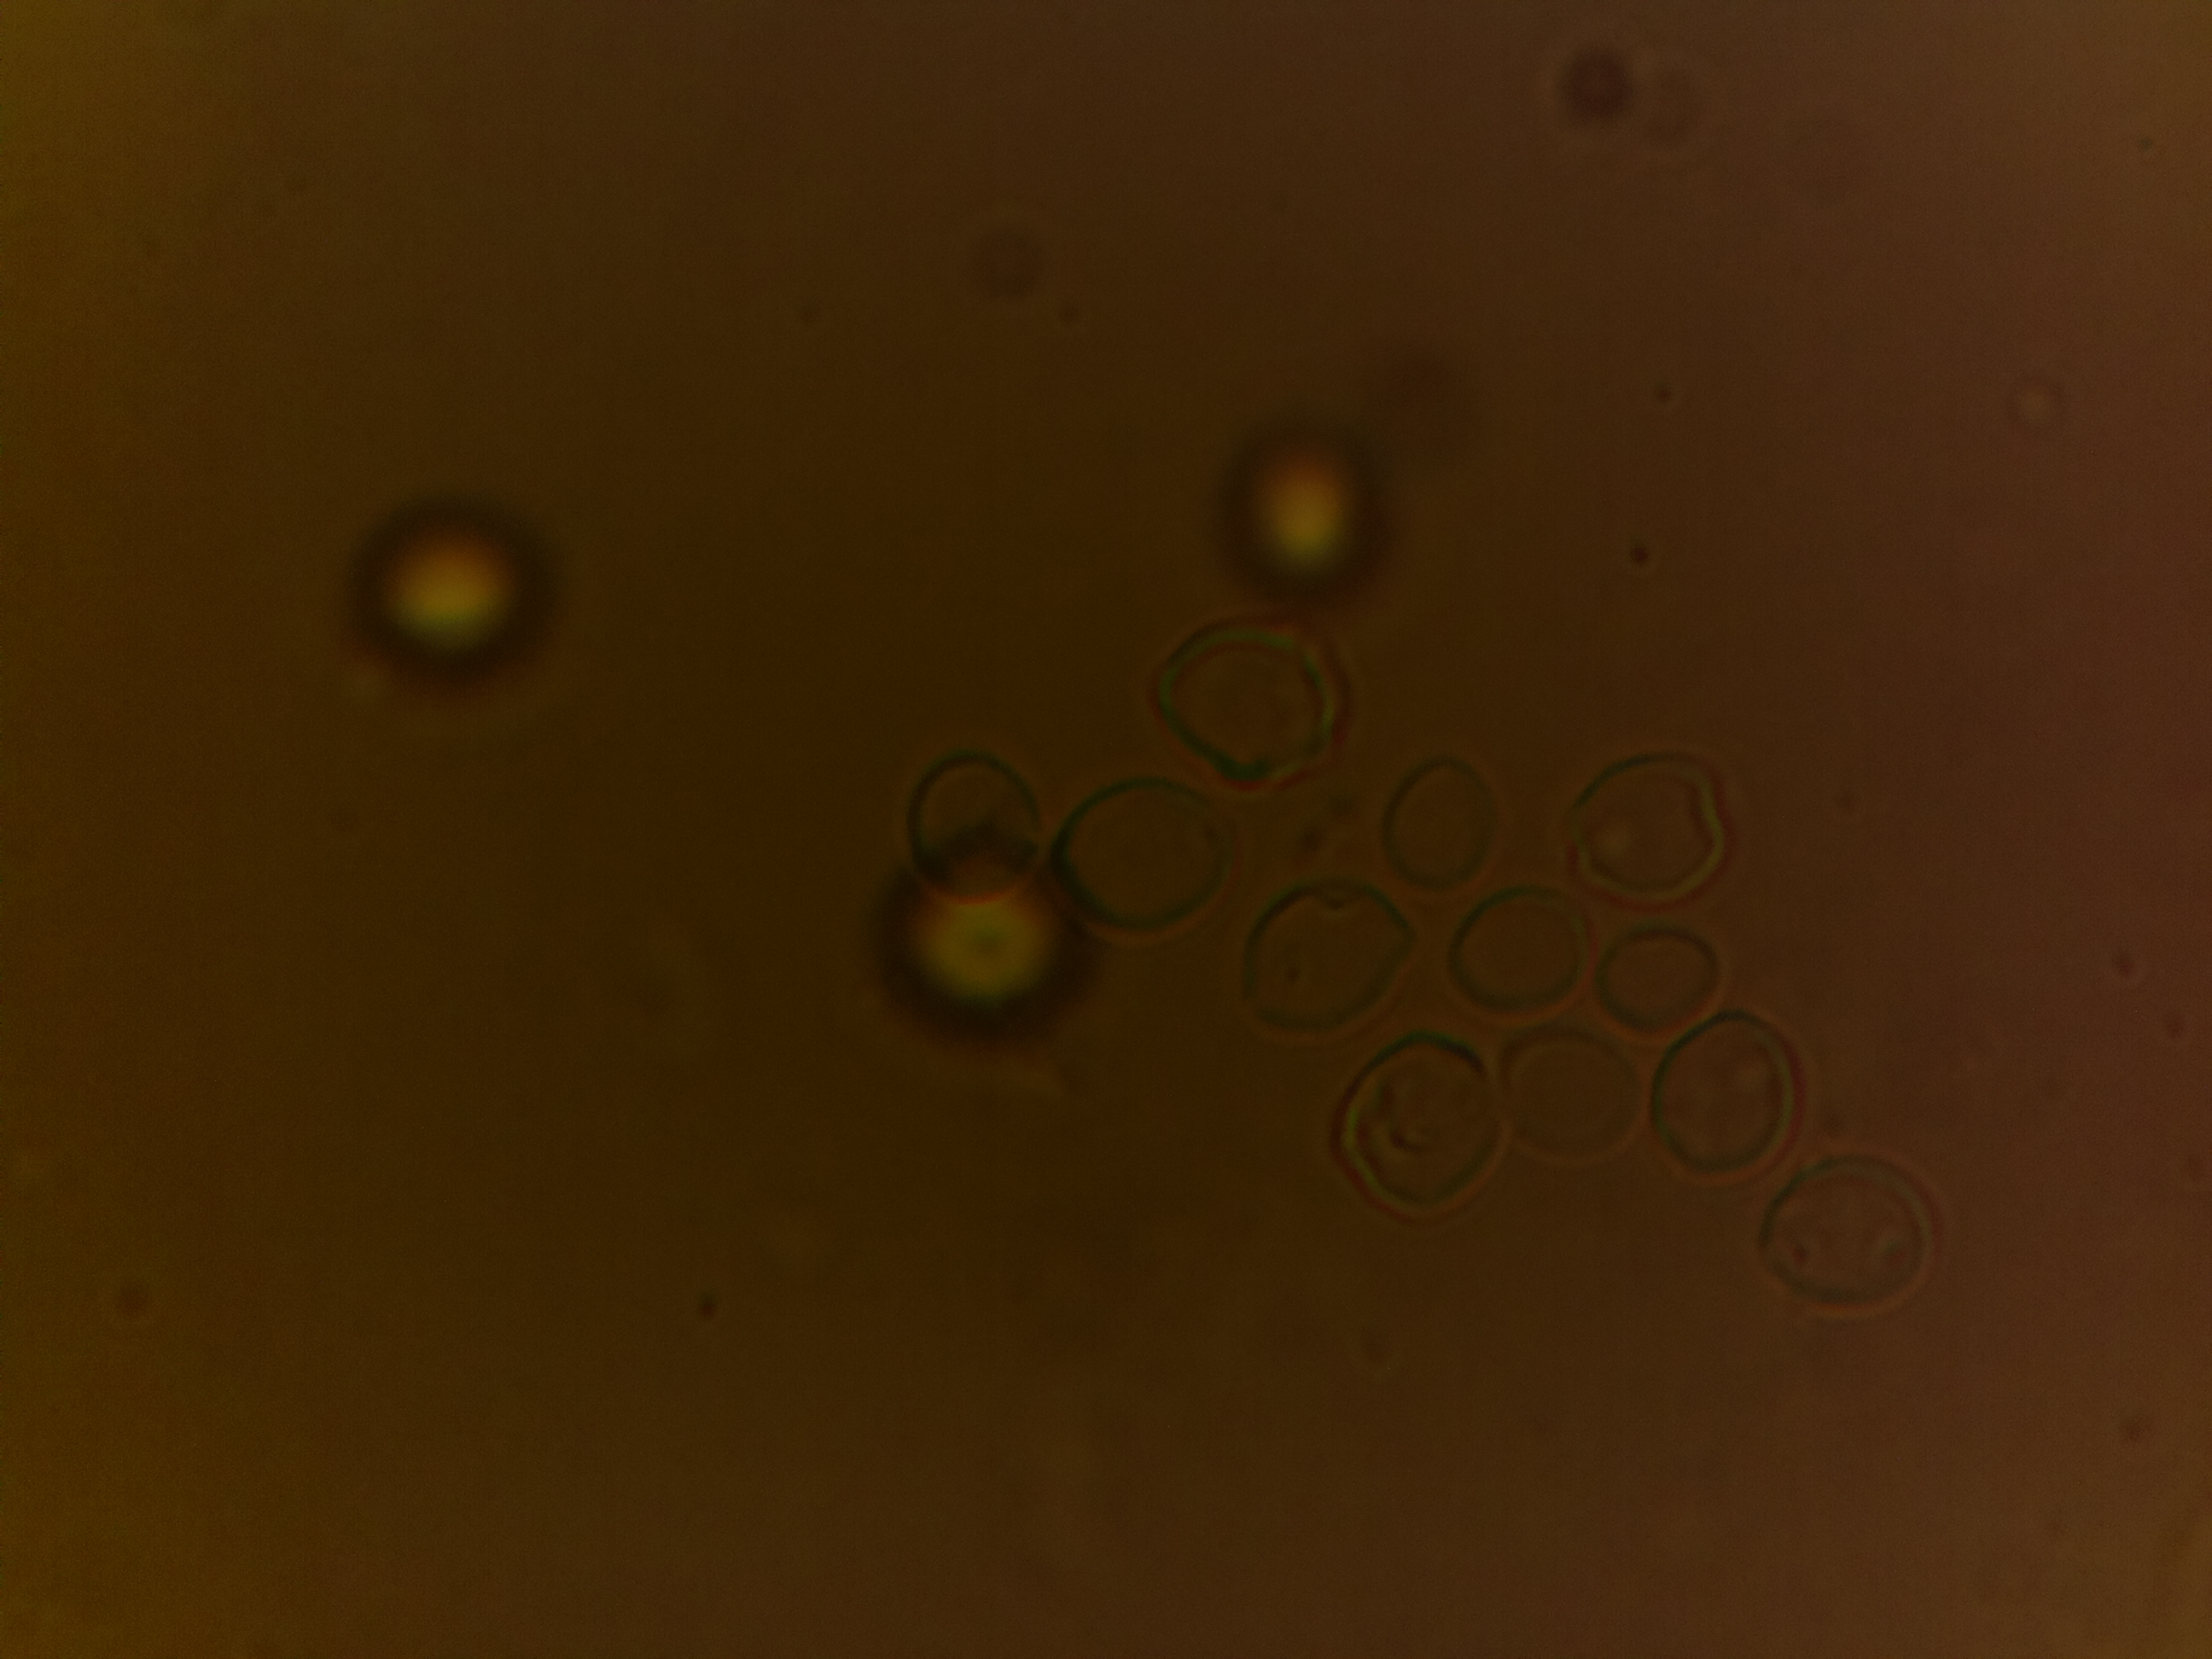
\includegraphics[width=10cm]{images/2016-03-30_185709.jpg}
\label{firstimage}
\caption{The first image in the sequence images/2016-03-30\_185709.jpg}
\end{center}
\end{figure}


\begin{figure}[th]
\begin{center}
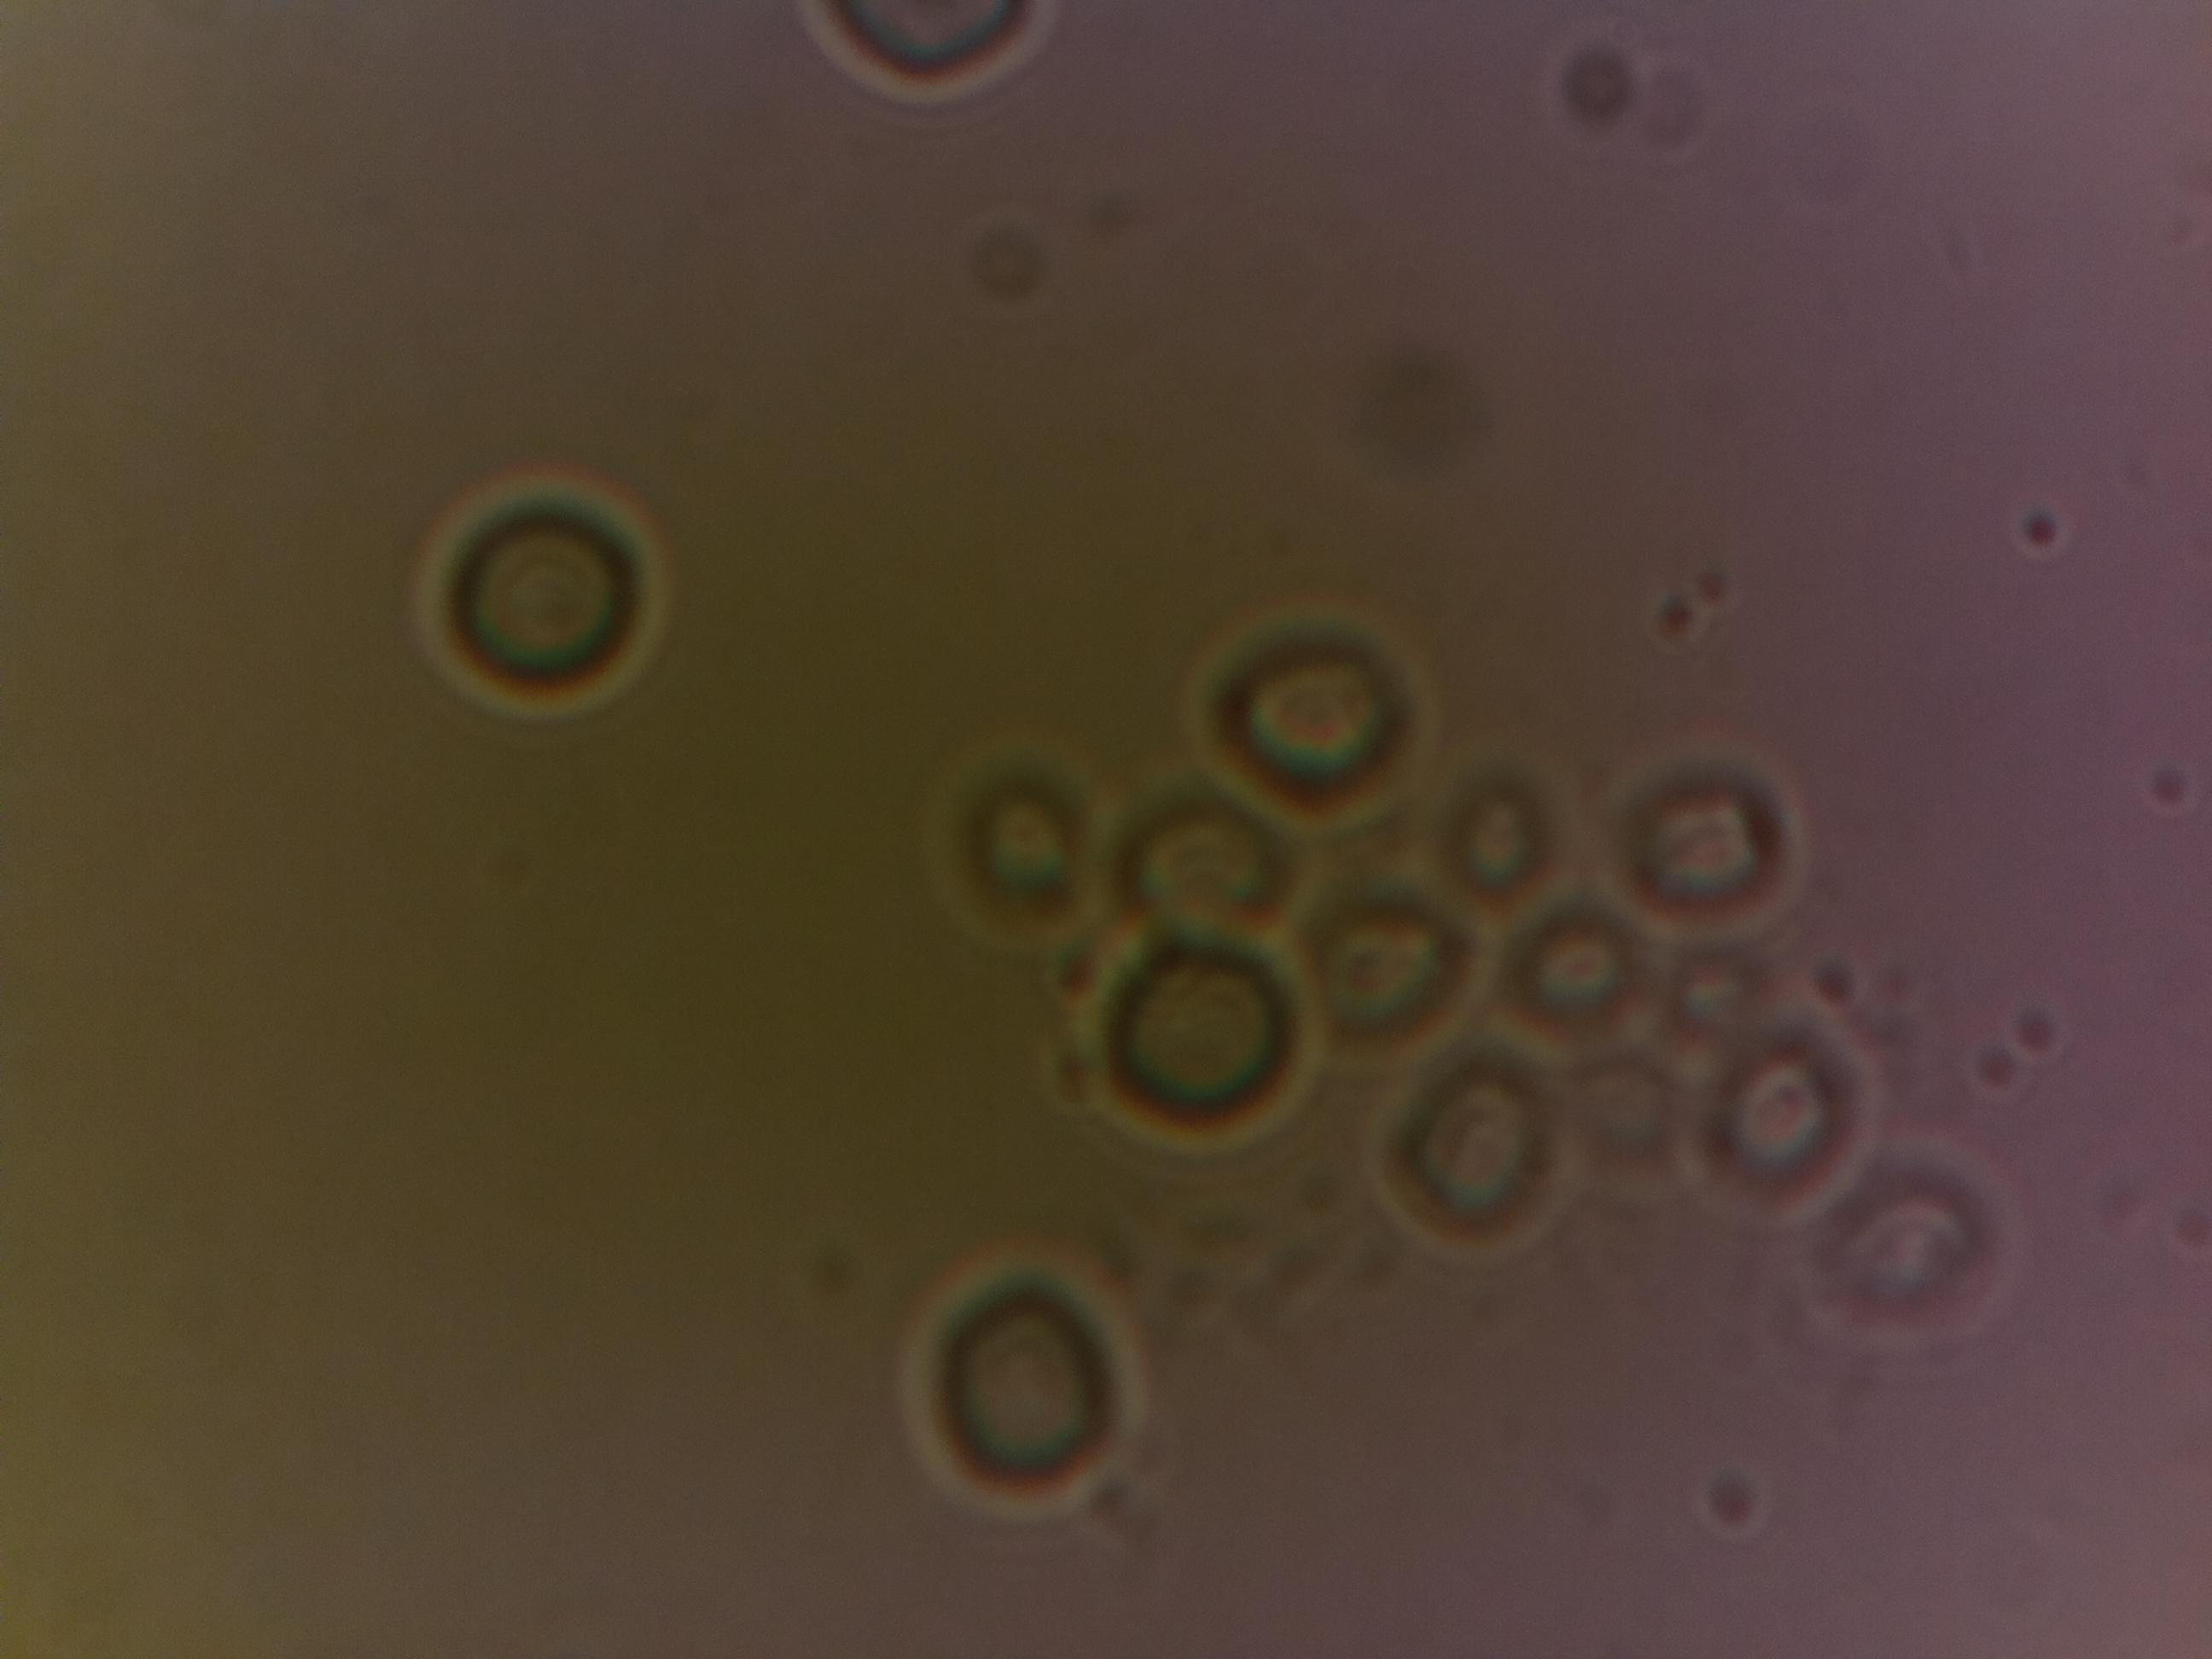
\includegraphics[width=10cm]{images/2016-03-30_203003.jpg}
\label{lastimage}
\caption{The last image in the sequence 2016-03-30\_203003.jpg}
\end{center}
\end{figure}


More images and an animation of the experiment can be found on the internet\footnote{An animation of the experiment: \url{https://dl.dropboxusercontent.com/u/187726/shared-experimental-data/yeast-growth-30-mar-2016/movies/yeast-growth.mp4}.}
\footnote{The raw image data: 
\url{https://dl.dropboxusercontent.com/u/187726/shared-experimental-data/yeast-growth-30-mar-2016/images}.}.


\section{Discussion}

It seems that the yeast died. Probably because of the high
temperature.  Try lower temperature next time.

There are bubbles floating by, it may be air or something else.   

Also, focus changes a lot during the experiment. It seems that
frequent focus adjustments are necessary to get high quality
animations over longer periods of time.



\section{References}


The previous experiment.


\end{document}
